% EN49 c08 | 原书 原书 p.76–86（PDF 87–97） | 第 5 章 §5.1–5.3
% 骨架文件：标题行已设定，正文由译者填写。每页起首用 % ===== 原书 p.N ===== 注释标记。
\section{镜像对称的应用}

% ===== 原书 p.76 =====
在下文关于镜像对称的应用中，我们将用到代数几何中的下述引理。证明相当简单，其梗概可见
[Sei08a, p.5]。设 $X$ 是光滑拟射影代数簇，$L$ 是带截面 $s$ 的线丛，并令
$U=X\setminus s^{-1}(0)$。

\begin{lemma}\label{lem:5-0-1}
设 $s\colon L^{-1}\otimes-\to\id$ 是由乘以截面 $s$ 给出的自然变换。则在 $s$ 处局部化
给出范畴等价
\[
\operatorname{Coh}(X)[s^{-1}]\simeq\operatorname{Coh}(U).
\]
\end{lemma}

\transnote{易错预警：原书此式印作 $s\colon L^{-1}\otimes\to\id$，$\otimes$ 后漏排了作用对
象；按上下文应读作自然变换 $L^{-1}\otimes-\to\id$，即对每个 $F$ 给出
$L^{-1}\otimes F\to F$。译文补上占位符「$-$」；原书在 p.80、p.85 还有两处同样的漏排，
译文一律照此处理，不再逐处注明。}

对这一引理的一种启发式解读是：局部化把镜像对称一侧「去掉一个除子」与另一侧「退化到特殊
纤维」联系了起来。

\transnote{背景直觉：引理 \ref{lem:5-0-1} 是全章的技术枢纽。B 侧去掉除子
$s^{-1}(0)$，等价于把相干层范畴在该截面给出的自然变换处局部化；A 侧沿同一自然变换局部
化，则得到奇异纤维的 Fukaya 范畴。两侧的局部化一旦对上，镜像对称就化归为光滑情形的已
知结论。}

% ===== 原书 p.77 =====
\subsection{裤子塔（tower of pants）}

Landau--Ginzburg 模型 $(\C^{n+1},W_n=z_1\cdots z_{n+1})$ 在镜像对称中具有特殊的重要
性：它是高维裤子 $\Pi_{n-1}=\{x_1+\cdots+x_n+1=0\}\subseteq(\C^*)^n$ 的镜像，例如见
[Nad19a; AAK16]。本节将借助 Abouzaid--Auroux 的工作 [AA21]，在这一特殊情形下勾勒镜像对
称与周期性的另一个证明。

\transnote{易错预警：裤子的下标等于变量个数减一。原书在本段写 $\Pi_{n-1}\subseteq
(\C^*)^n$（$n$ 个变量），到 p.78 又写 $\Pi_n\subseteq(\C^*)^{n+1}$（$n+1$ 个变量），两
处并不矛盾；第 1 章已把 $\Pi_n$ 定义为
$\{x_1+\cdots+x_{n+1}+1=0\}\subseteq(\C^*)^{n+1}$，与本段一致。}

对该 LG 模型，一般纤维 $W_n^{-1}(1)$ 由复环面 $(\C^*)^n$ 给出。我们知道它的 wrapped
Fukaya 范畴由单个拉格朗日量 $L=(\R_+)^n\subseteq(\C^*)^n$ 生成，自同态代数由
$\C[x_1^{\pm1},\dots,x_n^{\pm1}]$ 给出。我们将用到 Abouzaid--Auroux 宣布的下述结果：

\begin{thmstar}
（Abouzaid--Auroux [AA21]）\quad 范畴 $\cW(\C^{n+1},z_1\cdots z_{n+1})$ 由单个拉格朗
日量 $\cup L$ 生成。此外，该 LG 模型一般纤维上的 Seidel 自然变换 $s$ 对应态射
$L\to L$，由乘以 $x_1+\cdots+x_n+1$ 给出。
\end{thmstar}

\transnote{含糊点拨：原文说这两个结果由 Abouzaid--Auroux「announced」（宣布），即作者写作时
尚未正式成文，译本照译作「宣布」。$\cup$ 形符号另记由若干拉格朗日量经 cup 函子粘成的对
象，不是集合的并。例如 $\cup L$ 表示把 $L$ 沿 $\cup$ 函子的一份拷贝粘上去。}

自然变换中求和式 $x_1+\cdots+x_n+1$ 的每一项，对应经过该 LG 模型奇异纤维
$z_1\cdots z_{n+1}=0$ 中某个超平面 $z_i=0$ 的全纯曲线计数。

\begin{corollary}\label{cor:5-1-1}
存在范畴拟等价
\[
D^\pi\cW(W_n^{-1}(0))\simeq D^\pi\cW(\C^{n+2},z_1\cdots z_{n+2})\simeq
\operatorname{Coh}(\Pi_n).
\]
\end{corollary}

% ===== 原书 p.78 =====
\begin{figure}[htbp]
\centering
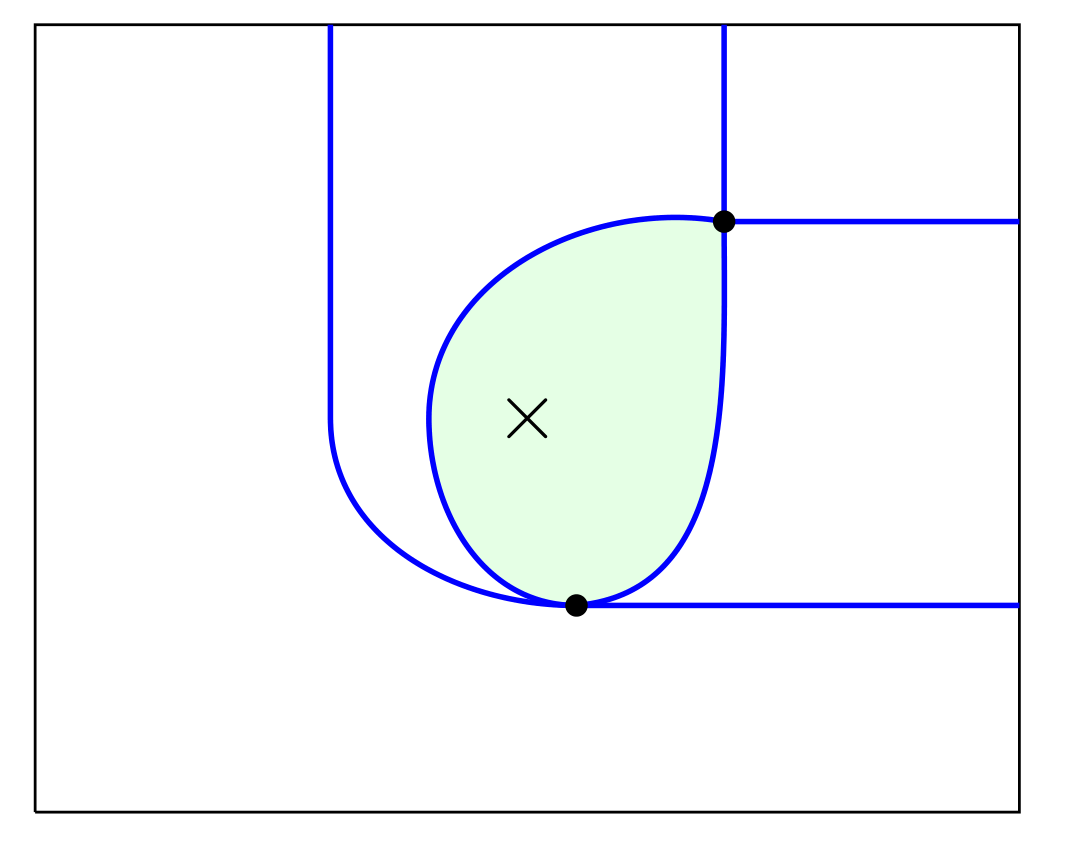
\includegraphics[width=0.38\textwidth]{figures/fig5_1.png}
\caption{计算一个 $\cup$ 形对象的自同态。}
\label{fig:5-1}
\end{figure}

\transnote{背景直觉：图 \ref{fig:5-1} 中的蓝色折线就是原文所称的 $\cup$ 形对象；绿色卵形区域
与两个黑点是辅助标记，图内没有公式或文字标注。证明里说把 $\cup L$ 推离自身，两个黑点正
是推离前后两份拷贝的交点，而自同态代数由该处的映射锥给出。}

\begin{proof}
利用局部化的定义，第一个范畴由 $\C[x_1^{\pm1},\dots,x_n^{\pm1}]$-模范畴在自然变换
$\id\to\id$ 处局部化给出，该自然变换由乘以 $x_1+\cdots+x_n+1$ 给出。这与下述范畴相
同：$\C$-代数 $\C[x_1^{\pm1},\dots,x_n^{\pm1}]$ 在 $x_1+\cdots+x_n+1$ 处局部化上的模
范畴，亦即 $\{x_1+\cdots+x_n+1\neq0\}\subseteq(\C^*)^n$ 上相干层的范畴；但后者恰是
$\{x_1+\cdots+x_n+1=-x_{n+1}\}\subseteq(\C^*)^{n+1}$，即裤子 $\Pi_n$。

第二个范畴可以通过计算生成元 $\cup L$ 的自同态得到。由于 $\cup L$ 由施加 $\cup$ 函子得
到，我们可以把它推离自身，从而看出其自同态代数由映射 $\End(L)\to\End(L)$ 的锥给出，而
该映射由乘以自然变换 $x_1+\cdots+x_{n+1}+1$ 给出（见图 \ref{fig:5-1}）。于是
$\cW(\C^{n+2},z_1\cdots z_{n+2})$ 由 $\C[x_1^{\pm1},\dots,x_{n+1}^{\pm1}]$ 对理想
$(x_1+\cdots+x_{n+1}+1)$ 取商后的模范畴给出。但后者恰是
$\{x_1+\cdots+x_{n+1}+1=0\}\subseteq(\C^*)^{n+1}$ 上相干层的范畴，即裤子 $\Pi_n$。
\end{proof}

应当可以把这一证明推广到环簇中超曲面的补集，按照 Abouzaid--Auroux 的想法，做法如下。设
$H\subseteq V$ 是环簇 $V$ 中的超曲面，由截面 $s\in\Gamma(V,\cO(H))$ 定义。

% ===== 原书 p.79 =====
$H\subseteq(\C^*)^n$ 的镜像由一个环簇 LG 模型 $(Y,W_Y)$ 给出 [Aur18]；把
$H\subseteq(\C^*)^n$ 紧化为 $H\subseteq V$ 会给超势增添额外的项，于是镜像是
$(Y,W_Y+\delta W)$：这里 $W$ 视为用于逐纤维缠绕的辅助超势，如 §4 所述。

\transnote{含糊点拨：secondary superpotential 译作「辅助超势」。它不改变 $Y$ 上原有的超
势 $W_Y$，只用来实现逐纤维的缠绕；$\delta W$ 是紧化时新增的项，其下标不加 $Y$，因为它是
$W$ 的修正而非 $W_Y$ 的修正。}

\begin{thmstar}
（Abouzaid--Auroux [AA21]）\quad 一般纤维的 Fukaya--Seidel 范畴
$D^\pi\cW(W_Y^{-1}(t),W)$ 拟等价于 $\operatorname{Coh}(V)$。此外，单值性 $\mu$ 在
$(W_Y^{-1}(t),W)$ 上的作用镜像于与线丛 $\cO(-H)$ 作张量，而自然变换 $\mu\to\id$ 镜像于
定义截面 $s\colon\cO(-H)\to\cO_V$。
\end{thmstar}

因此，我们的定义的一个 LG 版本使我们能断定：$D^\pi\cW(W_Y^{-1}(0),W)$ 等价于
$\operatorname{Coh}(V\setminus H)$，这里用到引理 \ref{lem:5-0-1}。此外，利用定义
\ref{def:sing-ci}，应当可以把这一点推广到 [AA21] 续篇所考虑的环簇中完全交的情形。

\transnote{易错预警：这里截面 $s$ 的方向是 $\cO(-H)\to\cO_V$，与引理 \ref{lem:5-0-1}
中 $L^{-1}\to\cO$ 的方向一致（$L=\cO(H)$）；若把 $s$ 看成 $\cO_V\to\cO(H)$，则论及的
是同一个截面的另一写法，局部化结论不变。}

\subsection{对曲线的应用}

定义 \ref{def:sing-fuk} 在实际计算中往往相当直接，下面的简单例子即可说明。

\begin{example}\label{exam:5-2-1}
考虑标准 Lefschetz 纤维丛 $X=\C^2$ 与 $f=xy$；我们直接计算结点二次曲线
$\{xy=0\}$ 的 Fukaya 范畴 $\cW(\{xy=0\})$。由引理 \ref{lem:2-3-1}，为求
$\cW(\{xy=0\})$，只需用 $\cap$ 的像对 $\cW(\{xy=t\})$ 取商。但在本例中，唯一能对之施
加 $\cap$ 的对象是 $(\C^2,xy)$ 的标准顶针，而 $\cap$ 恰好给出 vanishing cycle
$V\subseteq\{xy=t\}$。于是 $\cW(\{xy=0\})=\cW(\{xy=t\})/\langle V\rangle$。在
$D^\pi\cW(\{xy=t\})$ 与 $\operatorname{Coh}(\C^*)$ 的镜像对称下，$V$ 对应于点
$p\neq0$ 的点层，而商 $\operatorname{Coh}(\C^*)/\langle\cO_p\rangle$ 恰好给出
$\operatorname{Coh}(\C^*\setminus\{p\})$，它拟等价于裤子上的相干层
$\operatorname{Coh}(\Pi_1)$，这与前面的预期一致。
\end{example}

\transnote{易错预警：原书本例末尾印了一个证明结束符（$\square$），但正文中并没有 proof 环
境。译本把整段放在 example 环境内，不另立证明环境，也不补结束符；该处列入报告疑点。}

% ===== 原书 p.80 =====
在本例中，我们还可以利用 [LO06] 中 $A_\infty$ 范畴局部化的显式公式，计算
$\cW(\{xy=0\})$ 的完整 $A_\infty$ 结构。我们将在后续工作中对此多作讨论。

现在考虑亏格 $1$ 的带奇点曲线。考虑由椭圆曲线的 Tate 族给出的映射 $f\colon X\to\C$，
其中 $f^{-1}(0)$ 是带单个结点的椭圆曲线。由 [PZ01; LP12] 等的工作可知，一般纤维的
Fukaya 范畴 $\cF(f^{-1}(t))$ 与镜像椭圆曲线 $E$ 上的相干层范畴
$\operatorname{Coh}(E)$ 导出等价。此时绕该奇点的单值性由绕相应 vanishing cycle 的负
Dehn twist 扭转给出，它把镜像于 $\cO_E$ 的拉格朗日量 $L\subseteq f^{-1}(t)$，送到斜率
$(-1)$ 的拉格朗日量 $\mu(L)\subseteq f^{-1}(t)$，后者镜像于 $E$ 上次数 $(-1)$ 的线丛
$\cL^{-1}$ [PZ01]。由于单值函子由逐纤维平移到 $\mu(L)$ 给出，在这一镜像等价下，$\mu$
镜像于与线丛 $\cL^{-1}$ 作张量（讨论见下文 §5.3）。于是自然变换 $\mu\to\id$ 镜像于态
射 $\cL^{-1}\to\cO_E$，即对偶线丛 $\cL$ 的一个截面 $s$。因此，我们可以把
$\cW(f^{-1}(t))$ 在该自然变换处的局部化，与 $\operatorname{Coh}(E)$ 的局部化作比较。
一方面，由定义 \ref{def:sing-fuk}，$\cF(f^{-1}(t))$ 的这一局部化给出
$\cF(f^{-1}(0))$，即结点曲线的 Fukaya 范畴。在镜像一侧，由引理 \ref{lem:5-0-1}，
$\operatorname{Coh}(E)$ 在由乘以截面 $s$ 给出的自然变换 $\cL^{-1}\otimes-\to\id$ 处
的局部化，恰好给出补集的相干层导出范畴 $\operatorname{Coh}(E\setminus s^{-1}(0))$。

\transnote{含糊点拨：这里的单值函子「逐纤维平移到 $\mu(L)$」指在每个光滑纤维
$f^{-1}(t)$ 内把拉格朗日量平移，使平移量与 $\mu(L)$ 的截面一致；就范畴层面看，这只
改变了对象的位置，不改变其相交图。}

% ===== 原书 p.81 =====
于是我们得到结点椭圆曲线的 wrapped Fukaya 范畴，与单穿孔椭圆曲线的相干层导出范畴之间
的镜像等价。这一论证可以推广，以说明结点更多的椭圆曲线的 Fukaya 范畴，与穿孔数相应
的椭圆曲线导出等价：只需考虑 Gross--Siebert [GS03] 所论的椭圆曲线 $n$-结点退化的单值
性。

这一点还可以通过考虑带结点与穿孔的椭圆曲线加以推广：取 $f\colon X\to\C$ 为 $n$ 穿孔
椭圆曲线的仿射 Tate 族，其中 $f^{-1}(0)$ 是带单个结点与 $n$ 个穿孔的椭圆曲线。利用
[LP12; LP17] 对一般纤维的镜像等价，可以得到下述两族范畴之间的镜像导出等价。一侧是带
$n$ 个穿孔与 $m$ 个结点的椭圆曲线的 wrapped Fukaya 范畴，另一侧是带 $m$ 个穿孔与 $n$
个结点的椭圆曲线的相干层导出范畴（此处用到引理 \ref{lem:5-0-1} 的一个更强版本）。在本例中，由于 $f$
满足定理 \ref{thm:knorrer} 的假设，还有一个镜像等价：带 $m$ 个穿孔与 $n$ 个结点的椭圆
曲线的相干层，与 LG 镜像 $(X\times\C,zf)$ 的 Fukaya--Seidel 范畴等价。

\transnote{含糊点拨：「引理 \ref{lem:5-0-1} 的一个更强版本」指允许一次去掉多个除子的
情形，即对若干截面各自的自然变换同时局部化。原书未写出该版本，译本不补陈述。}

\subsection{推广}

上述椭圆曲线的例子，是更一般的大复结构极限与复环面同调镜像对称之间关系的一些特例。我
们先回顾 Gross--Siebert 在阿贝尔簇的环簇退化背景下的框架（见 [GS16, §2]）。

设 $M$ 是秩 $n$ 的格，$N=\Hom_\Z(M,\Z)$ 是对偶格，$\Gamma\subseteq M$ 是秩 $n$ 的子
格。商 $B=M_\R/\Gamma$ 自然带有整仿射流形的结构。

% ===== 原书 p.82 =====
设 $\cP$ 是 $M_\R$ 的 $\Gamma$-周期多面体分解，$\varphi\colon M_\R\to\R$ 是严格凸的
分段线性函数，其斜率为整数，且对任意 $\gamma\in\Gamma$ 有
\[
\varphi(m+\gamma)=\varphi(m)+\alpha_\gamma(m),
\]
其中 $\alpha_\gamma\colon M_\R\to\R$ 是某个整仿射函数。令 $\check\Gamma$ 为 $N_\R$ 中
的格 $\{\de\alpha_\gamma(m):\gamma\in\Gamma\}$；则商 $\check B=N_\R/\check\Gamma$ 也
带有整仿射流形的结构。离散 Legendre 变换（如 [GS06] 所述）给出 $N_\R$ 的对偶
$\check\Gamma$-周期多面体分解 $\check\cP$，以及严格凸的分段线性函数
$\check\varphi\colon N_\R\to\R$。令 $X(B)$ 为切丛对整向量子丛的商 $TB/T^\Z B$，令
$X^*(B)$ 为余切丛对整余向量子丛的商 $T^*B/T^*_\Z B$（对 $\check B$ 同样定义）。

\transnote{背景直觉：整仿射流形指局部上像 $\R^n$、坐标变换属
$\mathrm{GL}(n,\Z)\ltimes\R^n$ 的流形。$B$ 是底空间，$X(B)$ 与 $X^*(B)$ 分别是它上面
的「切丛模整向量」与「余切丛模整余向量」，二者在 Gross--Siebert 纲领中互为镜像的
B 模型与 A 模型。}

凸函数 $\varphi$ 通过 Mumford 构造的一个版本（[Mum72]，参见 [GS16, §2]）在 $X(B)$ 上
诱导一个丰富线丛 $\cL_\varphi$。$X(B)$ 上有一个自然复结构，该丰富线丛使 $X(B)$ 成为凯
勒流形，且与 $X^*(\check B)$ 上由余切丛 $T^*\check B$ 的典范辛形式给出的自然辛结构辛同
胚。我们可以把 $\cL_\varphi$ 显式构造成商 $M_\R\times\C/\Gamma$，其中
$\gamma\in\Gamma$ 的作用为
\[
\gamma\cdot(m,z)=(m+\gamma,\,z\,e^{\de\alpha_\gamma(m)+c_\gamma}),
\]
而 $c_\gamma$ 是差 $\alpha_\gamma(m)-\de\alpha_\gamma(m)$。Mumford 的这一构造给出
$X(B)$ 与 $X(\check B)$ 在单位圆盘 $D\subseteq\mathbb A^1$ 上的环簇退化
$\cX_\varphi\to D$ 与 $\check\cX_{\check\varphi}\to D$，它们构成 Gross--Siebert 镜像
对。大体积极限是补集 $X(B)\setminus s^{-1}(0)$，其中 $s$ 是丰富线丛 $\cL_\varphi$ 的截
面；

% ===== 原书 p.83 =====
而大复结构极限是环簇退化的中心纤维 $\cX^0_\varphi$。

\begin{thmstar}
（复述定理 \ref{thm:lvl-lcsl}）\quad 当 $B=M_\R/\Gamma$ 是整仿射环面，带有多面体分解
$\cP$，并取定严格凸分段线性多值函数 $\varphi$（其斜率为整）时，下述结论成立。大复结构
极限 $\check\cX^0_{\check\varphi}$ 同调镜像于大体积极限
$X(B)\setminus s^{-1}(0)$，即存在范畴的拟等价
\[
D^\pi\cF(\check\cX^0_{\check\varphi})\simeq\DBCoh(X(B)\setminus s^{-1}(0)).
\]
\end{thmstar}

\transnote{易错预警：原书此处把第 1 章的定理 \ref{thm:lvl-lcsl} 原样重述，并沿用原编号。译本
的编号全部自动生成，若另立有编号的定理环境，同一结论会得到「5.3.1」的新号，还会把后文
编号挤乱。故此处用无编号的 thmstar 环境，编号一律引定理 \ref{thm:lvl-lcsl}；后文重述定
理 1.4.2 同此处理。}

\begin{proof}[定理 \ref{thm:lvl-lcsl} 的证明]
该环簇退化的 Gross--Siebert 构造在 [GS06] 中具有如下性质：绕 $0$ 的（逆时针）单值性
$\check\mu^{-1}\colon X(\check B)\to X(\check B)$，由 $\check B$ 的展式映射的图作平移
给出 [GS10, p.79]。展式映射是从整仿射万有覆盖 $\tilde{\check B}$ 到 $N_\R$ 的整仿射
浸入 $\delta\colon\tilde{\check B}\to N_\R$，于是其图
$\sigma_1\subseteq\tilde{\check B}\times N_\R$ 在局部整仿射坐标下由 $(y,y)$ 给出
[GS06, p.13]。在 Legendre 变换下，$\check B$ 的展式映射由多值凸函数 $\varphi$ 在 $B$
上的微分 $\de\varphi\colon\tilde B\to N_\R$ 诱导 [GS06, p.14]。在 $X(\check B)$ 与
$X^*(B)$ 的等同下，$\check B$ 的展式映射的图由 $\de\varphi$ 在 $T^*B$ 中的图给出。

记 $(F_m,\xi)$ 为 $X^*(B)$ 在 $[m]\in M_\R$ 上的纤维，带 $U(1)$-局部系统 $\xi$，视为
Fukaya 范畴的对象。数对 $(m,\xi)$ 确定镜像 $X(B)$ 中的一点 $(m,\check\xi)$，其中
$\check\xi$ 是对偶局部系统。Abouzaid 的族 Floer 函子 [Abo17] 把 $X^*(B)$ 的零截面送到
结构层 $\cO_{X(B)}$，把 $X^*(B)$ 的截面 $L$ 送到 $X(B)$ 上的线丛 $\cL$。在该族 Floer
函子下，$\Gamma_{\de\varphi}$ 被送到 $X(B)$ 上的线丛 $\cL$，

% ===== 原书 p.84 =====
其中 Floer 复形 $\mathrm{CF}((F_m,\xi),\Gamma_{\de\varphi})$ 给出 $(m,\check\xi)\in
X(B)$ 处的茎。由于 $\Gamma_{\de\varphi}$ 是截面的图，交
$\Gamma_{\de\varphi}\cap F_m$ 由单个点 $x_m$ 组成。在族 Floer 构造下，
$(m,\check\xi)$ 与 $(m+\gamma,\check\xi)$ 处的茎通过换基点映射等同，该映射取
\[
x_m\mapsto x_{m+\gamma}\,e^{\int_{u_\gamma}\omega},
\]
其中 $u_\gamma$ 表示由零截面、纤维 $F_m$、$F_{m+\gamma}$ 与截面
$\Gamma_{\de\varphi}$ 围成的全纯多边形，如 [GS16, §2] 所述。由于 $X^*(B)$ 带有由
$T^*B$ 上典范 $1$-形式诱导的辛结构，图 $\Gamma_{\de\varphi}$ 下方的面积直接由下式给
出：
\[
\int_{u_\gamma}\omega=\int_{[m,m+\gamma]}\de\varphi
=\varphi(m+\gamma)-\varphi(m)=\alpha_\gamma(m)=\de\alpha_\gamma(m)+c_\gamma,
\]
而这些恰是 $\cL_\varphi$ 各纤维的过渡函数。因此族 Floer 函子把
$\Gamma_{\de\varphi}$ 送到 $\cL_\varphi$。此外，由于把拉格朗日量按 $X^*(B)$ 的截面
平移，在族 Floer 函子下对应与相应线丛 $\cL$ 作张量，该函子也把
$\Gamma_{k\,\de\varphi}$ 送到 $\cL_\varphi^{\otimes k}$。

\transnote{易错预警：原书在紧接的下一句把 $\Gamma_{\de\varphi}$ 印成
$\Gamma_{\de\phi}$，$\varphi$ 与 $\phi$ 混用；这是底本的排印不一致，二者是同一对象。译
文统一记作 $\Gamma_{\de\varphi}$，并把该处列入报告。}

Abouzaid 在 [Abo17] 中证明，族 Floer 函子给出 $\cF(X^*(B))$ 与 $\DBCoh(X(B))$ 的一个
满子范畴 $\cC$ 的等价。我们已经看到，该子范畴 $\cC$ 包含 $\cL_\varphi$ 及其全部幂。由
Orlov 的一个定理 [Orl09b, Theorem 4]，$\cL_\varphi$ 的各次幂分裂生成
$\DBCoh(X(B))$，故 $\DBCoh(X(B))$ 是 $\cC$ 的分裂闭包。因此，在族 Floer 函子下，
$\cF(X(\check B))$ 的分裂闭包等价于 $\DBCoh(X(B))$。由于单值性 $\check\mu$ 由被送到
线丛 $\cL_\varphi$ 的截面 $\Gamma_{\de\varphi}$ 作平移给出，族 Floer 函子把单值函子
$\check\mu^{-1}$ 送到与 $\cL_\varphi$ 作张量。

% ===== 原书 p.85 =====
因此，来自绕大复结构极限的单值性的 Seidel 自然变换 $\check\mu\to\id$，在我们选定的同
调镜像对称等价下，对应于由乘以某个截面 $s\colon\cO_{X(B)}\to\cL_\varphi$ 给出的自然变
换 $\cL_\varphi^{-1}\otimes-\to\id$。现在可以比较两侧的局部化：由引理
\ref{lem:5-0-1}，$\DBCoh(X(B))$ 在该自然变换处的局部化给出补集上的相干层
$\DBCoh(X(B)\setminus s^{-1}(0))$。由于 $s$ 是 $\cL_\varphi$ 的截面，除子
$s^{-1}(0)$ 对偶于凯勒形式 $\omega_{X(B)}$，于是 $X(B)\setminus s^{-1}(0)$ 是沿
$\omega_{X(B)}$ 的大体积极限。由于大复结构极限族的全空间光滑 [GS03, p.26]，在 A 侧，
由定义 \ref{def:sing-fuk} 可知，$\cF(X(\check B))$ 在由单值性给出的自然变换处的局部
化给出 $\cF(\check\cX^0_{\check\varphi})$，即奇异中心纤维的 Fukaya 范畴。于是我们得到
大复结构极限与大体积极限之间的同调镜像对称拟等价：
\[
D^\pi\cF(\check\cX^0_{\check\varphi})\simeq\DBCoh(\check X\setminus s^{-1}(0)).
\]
\end{proof}

\transnote{易错预警：末式右侧原书印作 $\check X\setminus s^{-1}(0)$，与定理陈述中的
$X(B)\setminus s^{-1}(0)$ 不同。$\check X$ 应指 $X(\check B)$，也可能指退化的全空间
$\check\cX$；底本在此未作说明。译文照录 $\check X$，不改动，并把这一处列入报告。}

沿用上述证明的最后几步，我们还有下述条件性结果：

\begin{thmstar}
（复述定理 \ref{thm:lcsl}）\quad 给定 $X(B)$ 与 $X(\check B)$ 之间的同调镜像对称等
价。设它把绕 $X(\check B)$ 的大复结构极限的（顺时针）单值函子 $\mu$ 与 $X(B)$ 上线丛
$\cL^{-1}$ 的张量积等同起来，且 $\cL$ 的第一 Chern 类 $c_1(\cL)$ 就是 $X(B)$ 上凯勒形
式所在的类。则 $X(\check B)$ 的大复结构极限 $X_0(\check B)$ 同调镜像于 $X(B)$ 的某个
大体积极限：
\[
D^\pi\cF(X_0(\check B))\simeq\DBCoh(X(B)\setminus s^{-1}(0)),
\]
其中 $s$ 是 $\cL$ 的截面。
\end{thmstar}

% ===== 原书 p.86 =====
要应用定理 \ref{thm:lcsl}，需要上述形式的同调镜像对称等价。在拉格朗日环面丛带奇点的情
形，预期可以把 Abouzaid 的族 Floer 理论与 Gross--Siebert 纲领的想法结合起来（参见
[GS16]），按与上面相同的方式得到这种等价。在映射
$\tilde B\times M_\R\mapsto TB/T^\Z B$ 下，展式映射被送到截面
\[
y\mapsto\sum_{i=1}^n y_i\frac{\partial}{\partial y_i},
\]
它恰是 [GS16] 中描述的典范截面 $\sigma_1$。在 [GS16, §4] 中已有说明：族 Floer 函子应
把 $\sigma_1$ 的图送到给出镜像上凯勒形式的丰富线丛 $\cL_\varphi$ 的逆。

\transnote{背景直觉：$\sigma_1$ 是切丛里的典范截面
$y\mapsto\sum_i y_i\partial/\partial y_i$，也称 Euler 向量场。它的图在族 Floer 函子下
应对应丰富线丛之逆，这与前文 $\Gamma_{\de\varphi}$ 对应 $\cL_\varphi$ 的机制相同，只
是符号相反。}

因此，在对定义 \ref{def:sing-fuk} 作适当修改之后，类似定理 \ref{thm:lvl-lcsl} 的结果
在这一情形也应成立。
